\documentclass{article}

% VLM4RWD 2026 (2nd Workshop on Grounded and Faithful Vision-Language Models
% for Real-World Deployment), NeurIPS 2026, Sydney. Double-blind, 8 pages
% excluding references/appendices, non-archival. Camera-ready: add `final`.
\usepackage[dblblindworkshop]{neurips_2026}

\usepackage[utf8]{inputenc}
\usepackage[T1]{fontenc}
\usepackage{hyperref}
\usepackage{url}
\usepackage{booktabs}
\usepackage{amsfonts}
\usepackage{amssymb}
\usepackage{amsmath}
\usepackage{nicefrac}
\usepackage{microtype}
\usepackage{graphicx}
\usepackage{xcolor}
\usepackage{tikz}
\usetikzlibrary{arrows.meta,positioning,fit,calc}

\graphicspath{{figures/}}
\newcommand{\hitat}[1]{hit@#1}
\newcommand{\mix}[1]{\texttt{#1}}

\workshoptitle{2nd Workshop on Grounded and Faithful Vision-Language Models for Real-World Deployment (VLM4RWD)}

\title{Decoupling What from Where: Action-Type Supervision for GUI Grounding in a Small Vision-Language Model}

\author{Anonymous Author(s)}

\begin{document}

\maketitle

\begin{abstract}
A GUI agent has to decide which action to take (click, scroll, type) and where on the screen to take it. Native agent models emit both decisions in one token stream. We ask whether separating them improves grounding, using Qwen2-VL-2B with LoRA on Android in the Wild and Multimodal-Mind2Web. Stage~1 classifies the action type from frozen features; Stage~2 predicts a coordinate and can be conditioned on the type through one of four mechanisms, compared with a flat baseline under matched data, compute, and decoding. With five seeds and paired bootstrap tests over 1,250 examples, an auxiliary action-type loss and an additive learned embedding each raise \hitat{0.10} by 5 to 6 points over the flat baseline when the action type predicts the target location, and change nothing on a control mix where it does not. A prepended learned action token, the mechanism we originally hypothesized, is no better than the baseline. Intervention experiments explain the difference: the additive embedding can be zeroed at test time without loss, so its benefit is a training effect, whereas the prepended token is used at inference and still does not help. Across training sizes from 300 to 5,000 examples, only the additive mechanism helps consistently. We also document a positional-encoding pitfall: injecting the conditioning through \texttt{inputs\_embeds} bypasses Qwen2-VL's M-RoPE and produced an apparent ten-point deficit that vanished once the \texttt{input\_ids} path was preserved.
\end{abstract}

\section{Introduction}
\label{sec:intro}

A GUI agent maps a screenshot and an instruction to a low-level action: an action type such as \emph{click}, \emph{scroll}, or \emph{type}, and, for spatial actions, a target location. Current native agent models (UI-TARS~\citep{uitars}, OS-Atlas~\citep{osatlas}, SeeClick~\citep{seeclick}, ShowUI~\citep{showui}) produce both in a single autoregressive stream. The two decisions are different kinds of prediction, though. The action type is a small classification problem that depends on the goal and the screen state; the location is a localization problem, in which the model has to find the evidence on the screen that supports the action and commit to a point. When a joint decoder gets the type wrong, it tends to ground consistently within the wrong choice, scrolling past a visible button instead of clicking it. The action is locally coherent and globally wrong, and on multi-step tasks the error compounds because the screen state changes.

This paper asks a narrow question about that failure mode: does telling the grounding model which action it is grounding improve where it grounds? We build a two-stage pipeline around Qwen2-VL-2B~\citep{qwen2vl}. Stage~1 predicts the action type from mean-pooled frozen features with a small MLP. Stage~2 fine-tunes the backbone with LoRA~\citep{lora} to emit a coordinate string and receives the action type through one of four conditioning mechanisms: an auxiliary classification loss, a hard-routed action word in the output, an additive learned embedding, and a prepended learned action token. Each is compared with a flat baseline that sees the same data and uses the same optimizer, adapters, and decoding. We started from the hypothesis that the prepended token would be the right mechanism, because it gives the model a dedicated, attendable position for the action type.

The evidence supports the factorization and refutes our hypothesis about the mechanism. On an Android in the Wild mix where the action type predicts the target location, the auxiliary loss and the additive embedding improve \hitat{0.10} over the flat baseline by $+0.064$ and $+0.054$ (five seeds, paired bootstrap over 1,250 examples, $p<0.001$), and the two are indistinguishable from each other. On a control mix of taps and swipes, where the type carries no spatial information, neither differs from the baseline. The prepended token is within noise of the baseline and worse than the auxiliary loss. Across training sizes from 300 to 5,000 examples, the additive embedding is the only mechanism that helps at nearly every size; the auxiliary loss helps at some sizes and hurts at one. Intervention experiments on the trained models explain the ranking: the additive embedding can be zeroed at test time with no loss in accuracy, so its benefit comes from training, whereas the prepended token is used at inference and still does not help. The same study surfaced a silent failure. An earlier implementation injected the conditioning through \texttt{inputs\_embeds}, which bypasses Qwen2-VL's multimodal rotary position computation; that version scored ten points below the baseline, and keeping the \texttt{input\_ids} path removed the deficit entirely.

Our contributions are: (1) a matched-compute comparison of four conditioning mechanisms against a flat baseline on two GUI datasets, with five-seed paired statistics and a control mix where conditioning should not help; (2) a scaling study from 300 to 5,000 examples with three seeds per size; (3) interventions and attention measurements that separate training-time from inference-time use of the signal; and (4) a positional-encoding pitfall that produced a large false negative.

\section{Related Work}
\label{sec:related}

\paragraph{GUI grounding and agent models.}
Mind2Web~\citep{mind2web} and Android in the Wild~\citep{aitw} supply the web and mobile episodes we train on; AndroidControl~\citep{androidcontrol} and AndroidWorld~\citep{androidworld} extend mobile evaluation. SeeClick~\citep{seeclick} argued that grounding is the bottleneck for visual GUI agents and introduced ScreenSpot; ScreenSpot-Pro~\citep{screenspotpro} raises the resolution. UGround~\citep{uground} and OS-Atlas~\citep{osatlas} scale grounding pretraining, and Aguvis~\citep{aguvis}, UI-TARS~\citep{uitars}, CogAgent~\citep{cogagent}, ScreenAI~\citep{screenai}, and Ferret-UI~\citep{ferretui} train agents that emit action and location together, the design our flat baseline follows. GUI-Actor~\citep{guiactor} replaces coordinate text with an attention-based action head, UI-R1~\citep{uir1} rewards the action type and the argument separately, RegionFocus~\citep{regionfocus} zooms at test time, and OmniParser~\citep{omniparser} and Set-of-Mark prompting~\citep{som} externalize grounding into a parser. SeeAct~\citep{seeact}, Ponder\,\&\,Press~\citep{ponderpress}, and Aria-UI~\citep{ariaui} separate text planning from pixel grounding; our boundary is between the action type and the location. GUI-Libra~\citep{guilibra} adds action-aware supervision and GUI-AIMA~\citep{guiaima} an anchor token, close in spirit to our auxiliary-loss and prepended-token variants, without the mechanism-level interventions we run.

\paragraph{Conditioning and factorized decision-making.}
SayCan~\citep{saycan} separates what a language model wants to do from what the environment affords; ReAct~\citep{react} exposes intermediate decisions as text; RT-2~\citep{rt2} is the reference for emitting actions as tokens. On the same mobile benchmark we use, AutoUI~\citep{autoui}, AppAgent~\citep{appagent}, DigiRL~\citep{digirl}, WebRL~\citep{webrl}, and VSC-RL~\citep{vscrl} improve agents by imitation or reinforcement learning without changing how the action type enters the grounding computation. Our auxiliary-loss variant is a multi-task objective in the sense of \citet{caruana}.

\paragraph{Grounded and faithful VLMs.}
Kosmos-2~\citep{kosmos2}, Shikra~\citep{shikra}, and Ferret~\citep{ferret} train VLMs to refer to image regions, and POPE~\citep{pope} and HallusionBench~\citep{hallusionbench} measure whether a model's output is supported by the image. GUI grounding is a deployment-shaped instance of the same question: the coordinate is only correct if the model found the evidence for it on the screen. Our attention measurements ask directly whether the conditioning signal moves the model's evidence toward the target.

\paragraph{Backbone and adaptation.}
Qwen2-VL~\citep{qwen2vl} assigns three-dimensional rotary positions (M-RoPE, an extension of RoPE~\citep{roformer}) to visual tokens, and the assignment is keyed off \texttt{input\_ids}; Section~\ref{sec:mrope} shows what happens when conditioning is injected around that path. All fine-tuning uses LoRA~\citep{lora}.

\section{Method}
\label{sec:method}

\begin{figure}[t]
  \centering
  \resizebox{\linewidth}{!}{% Architecture figure: two-stage factorization + the six Stage-2 conditioning
% mechanisms. \input from main.tex inside a figure environment.
% Requires: \usepackage{tikz} with libraries arrows.meta, positioning, fit, calc.
% Natural width is about 13.5 cm so that \resizebox{\linewidth} scales it by ~1.
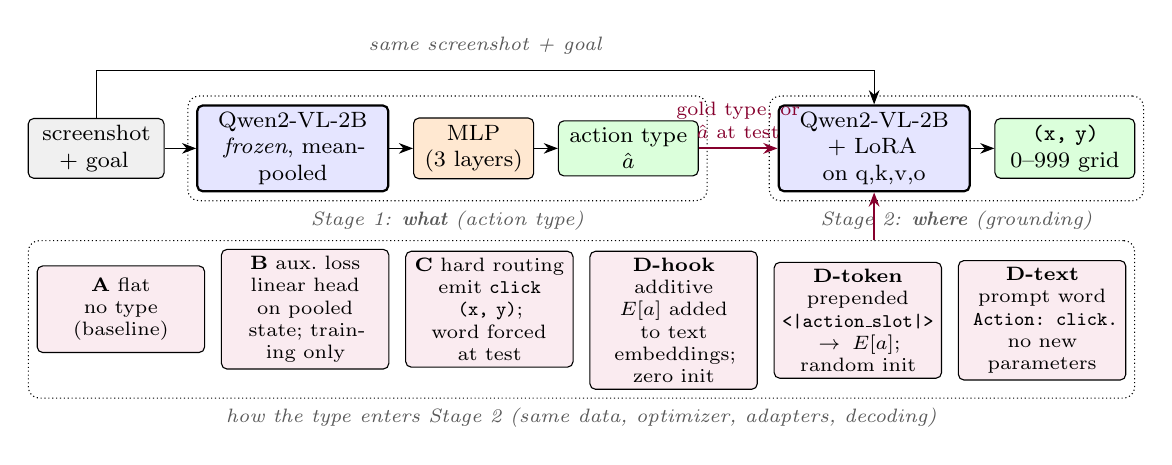
\begin{tikzpicture}[
  font=\footnotesize,
  >={Stealth[length=1.8mm]},
  box/.style={draw, rounded corners=2pt, align=center, inner sep=2.5pt, minimum height=7mm},
  inp/.style={box, fill=gray!12, text width=1.55cm},
  model/.style={box, fill=blue!10, thick, text width=2.25cm},
  head/.style={box, fill=orange!18, text width=1.35cm},
  outp/.style={box, fill=green!14, text width=1.6cm},
  mech/.style={box, fill=purple!8, text width=1.95cm, minimum height=11mm, font=\scriptsize},
  lbl/.style={font=\scriptsize\itshape, text=black!65},
  cond/.style={->, thick, purple!70!black},
  node distance=3mm,
]
  % ---------------- pipeline row ----------------
  \node[inp] (shot) {screenshot\\ + goal};
  \node[model, right=4mm of shot] (vlm1) {Qwen2-VL-2B\\ \textit{frozen}, mean-pooled};
  \node[head, right=of vlm1] (mlp) {MLP\\ (3 layers)};
  \node[outp, right=of mlp] (atype) {action type\\ $\hat a$};
  \node[model, right=10mm of atype] (vlm2) {Qwen2-VL-2B\\ + LoRA on q,k,v,o};
  \node[outp, right=of vlm2] (coord) {\texttt{(x, y)}\\ 0--999 grid};
  \node[draw, densely dotted, rounded corners, inner sep=3pt, fit=(vlm1)(mlp)(atype),
        label={[lbl]below:{Stage 1: \textbf{what} (action type)}}] (s1) {};
  \node[draw, densely dotted, rounded corners, inner sep=3pt, fit=(vlm2)(coord),
        label={[lbl]below:{Stage 2: \textbf{where} (grounding)}}] (s2) {};
  \draw[->] (shot) -- (vlm1);
  \draw[->] (vlm1) -- (mlp);
  \draw[->] (mlp) -- (atype);
  \draw[->] (vlm2) -- (coord);
  \draw[cond] (atype) -- node[above, font=\scriptsize, text=purple!70!black, align=center]
    {gold type, or\\ $\hat a$ at test} (vlm2);
  % the same inputs feed Stage 2, routed over the top
  \draw[->] (shot.north) -- ++(0,6mm) -| (vlm2.north);
  \node[lbl, anchor=south] at ($(shot.north)!0.5!(vlm2.north) + (0,6mm)$) {same screenshot + goal};

  % ---------------- mechanism row ----------------
  \coordinate (mid) at ($(shot.west)!0.5!(coord.east)$);
  \node[mech, anchor=north east] (C) at ($(mid) + (-1mm,-13mm)$)
    {\textbf{C} hard routing\\ emit \texttt{click (x, y)};\\ word forced at test};
  \node[mech, anchor=north west] (Dh) at ($(mid) + (1mm,-13mm)$)
    {\textbf{D-hook} additive\\ $E[a]$ added to text\\ embeddings; zero init};
  \node[mech, left=2mm of C] (B)
    {\textbf{B} aux.\ loss\\ linear head on pooled\\ state; training only};
  \node[mech, left=2mm of B] (A)
    {\textbf{A} flat\\ no type\\ (baseline)};
  \node[mech, right=2mm of Dh] (Dt)
    {\textbf{D-token} prepended\\ \texttt{<|action\_slot|>}\\ $\to E[a]$; random init};
  \node[mech, right=2mm of Dt] (Dx)
    {\textbf{D-text} prompt word\\ \texttt{Action: click.}\\ no new parameters};
  \node[draw, densely dotted, rounded corners, inner sep=3pt, fit=(A)(B)(C)(Dh)(Dt)(Dx),
        label={[lbl]below:{how the type enters Stage 2 (same data, optimizer, adapters, decoding)}}] (fitbox) {};
  \draw[cond] (fitbox.north -| vlm2.south) -- (vlm2.south);
\end{tikzpicture}
}
  \caption{Two-stage pipeline. Stage~1 classifies the action type from mean-pooled frozen features. Stage~2 grounds the action to a coordinate string, and the action type enters it through one of the mechanisms in the bottom row. All mechanisms share data, compute, adapters, and decoding. D-slot is the retracted variant whose \texttt{inputs\_embeds} injection bypassed M-RoPE.}
  \label{fig:arch}
\end{figure}

\subsection{Action taxonomy and grounding target}
Both datasets are mapped onto a canonical eight-class action space (\emph{click}, \emph{double-click}, \emph{type}, \emph{scroll}, \emph{drag}, \emph{hotkey}, \emph{wait}, \emph{finished}). Mind2Web's CLICK, SELECT, and HOVER map to \emph{click} and TYPE to \emph{type}. AITW stores most actions as dual-point gestures; we split them into taps (\emph{click}) and swipes (\emph{scroll}) by the normalized distance between touch and lift, with threshold 0.04. The grounding target is the touch point normalized to $[0,1]^2$, serialized as the string \texttt{(x, y)} with integers on a $0$--$999$ grid, so every target has the same token length.

\subsection{Stage 1: which action}
Stage~1 runs the frozen Qwen2-VL-2B-Instruct backbone over the screenshot and instruction, mean-pools the final hidden states over unmasked tokens into a 1536-dimensional vector, and trains a three-layer MLP ($1536 \to 1024 \to 256 \to 8$, dropout 0.1) with class-weighted cross-entropy, AdamW (learning rate $10^{-4}$, weight decay 0.01), batch size 128, for eight epochs, keeping the checkpoint with the best validation macro-F1. We compare features from text only, text plus screenshot, and a sanity variant with zeroed features.

\subsection{Stage 2: where}
Stage~2 fine-tunes the same backbone with LoRA adapters (rank 16, $\alpha=32$, dropout 0.05) on the query, key, value, and output projections, 4.4M trainable parameters out of 2.2B (0.2\%). The prompt is the screenshot followed by \texttt{Goal: \{goal\}} and a fixed instruction to predict the action coordinate; the answer is the coordinate string. Let $s$ be the screenshot, $g$ the goal, $a$ the action type, and $y_{1:T}$ the coordinate tokens. Every variant minimizes
\begin{equation}
  \mathcal{L}_{\mathrm{coord}} = -\sum_{t=1}^{T} \log p_\theta\big(y_t \mid y_{<t},\, s,\, g,\, c\big),
  \label{eq:coord}
\end{equation}
with the loss masked to the answer tokens and $c$ the variant-specific conditioning.

\textbf{A, flat.} $c=\varnothing$. This is the joint-decoding design of native agent models, reduced to the grounding sub-problem.

\textbf{B, auxiliary loss.} A linear head $h_\phi$ on the mean-pooled last hidden state $\bar z$ predicts the action type during training, $\mathcal{L}_{\mathrm{B}} = \mathcal{L}_{\mathrm{coord}} + \lambda\,\mathrm{CE}(h_\phi(\bar z), a)$ with $\lambda=1$. Nothing about the action type is provided at inference, so any gain is a training effect.

\textbf{C, hard routing.} The model is trained to emit the action word before the coordinate, \texttt{click (x, y)}. At test time the word for the gold (or Stage-1) type is forced as a decoding prefix and the model completes the coordinate.

\textbf{D-hook, additive embedding.} A learned table $E \in \mathbb{R}^{8\times d}$ holds one vector per class. A forward hook on the embedding layer adds $E[a]$ to every token embedding. $E$ is zero-initialized, so D-hook starts as an exact copy of A and can only depart from it by learning to use the signal.

\textbf{D-token, prepended action token.} A new token \texttt{<|action\_slot|>} is added to the vocabulary and placed at the start of the text prompt, so it occupies a real position in \texttt{input\_ids} and M-RoPE treats it like any other token. A forward hook replaces the embedding at that position with $E[a]$. This is the architecture we originally hypothesized: a full-norm, attendable representation of the action type.

For C, D-hook, and D-token the gold type is used during training and at evaluation unless stated otherwise; Section~\ref{sec:e2e} closes the loop with Stage-1 predictions. All variants share the data order, the optimizer (AdamW, learning rate $2\times10^{-5}$, weight decay 0.01, batch size 1, gradient clipping at 1.0, two epochs), and greedy decoding with 16 new tokens.

\section{Experimental setup}
\label{sec:setup}

\paragraph{Data.}
Stage~1 uses 7,775 Multimodal-Mind2Web training steps evaluated on the 1,338-step \texttt{test\_task} split, and 5,000 AITW steps evaluated on 1,000 held-out steps. Stage~2 uses two AITW mixes. \mix{all\_with\_coords} contains taps, swipes, and type events; the validation slice of 250 steps has 169 clicks, 46 scrolls, and 35 type events, so the action type is informative about location. \mix{taps\_and\_swipes} contains only taps and swipes (1,000 training and 200 validation steps); both land anywhere on the screen, so the type carries no spatial information; this mix is the control. A second control uses Multimodal-Mind2Web (1,000 training and 250 evaluation steps), where the target is the center of the gold element and we also report whether the predicted point falls inside the element's box. The AITW stream is deterministic, so for a given mix and training size every seed and every variant is evaluated on the same examples in the same order. The validation slice starts where the training slice ends, which means absolute numbers are not comparable across training sizes; only within-size differences are.

\paragraph{Metrics and statistics.}
\hitat{r} is the fraction of predictions within normalized Euclidean distance $r$ of the target, for $r \in \{0.05, 0.10, 0.25\}$; \hitat{0.10} is the headline. We also report the mean normalized distance. Unparseable outputs count as misses at distance $\sqrt{2}$. The headline mix uses five seeds (42 to 46), all other cells three (42 to 44); we report mean and sample standard deviation over seeds. Because every run logs a per-example distance on a shared evaluation set, we test differences with a paired bootstrap over pooled (seed, example) units, matching seeds by id: 10,000 resamples, 95\% percentile intervals, and a two-sided bootstrap $p$-value~\citep{efron}. A paired permutation test agrees in every case we report. Stars denote $p<0.05$, $0.01$, and $0.001$.

\section{Results}
\label{sec:results}

\subsection{Stage 1: the screenshot decides the action type on AITW}
Stage~1 (Table~\ref{tab:stage1} in the appendix, three seeds) sets up the rest of the paper. On Mind2Web the instruction usually contains the action word: a bag-of-words classifier reaches 0.622 macro-F1, the frozen VLM features 0.605, and the screenshot is worth $+0.009$. On AITW the instruction is a goal (``open a new private window''), text-only features sit at the majority-class floor (0.141), and the screenshot is worth $+0.414$ macro-F1 (0.555). Predicting the action type is a vision problem on AITW, which is why the Stage-2 study is run there and why Mind2Web is used as a control.

\subsection{Conditioning helps where the action type predicts the location}
\label{sec:headline}

\begin{table}[t]
\centering
\small
\caption{Stage 2 grounding on AITW \texttt{all\_with\_coords} (n$_{\text{train}}$=1200, n$_{\text{val}}$=250, 5 seeds). Mean $\pm$ std over seeds; $\Delta$ with 95\% paired-bootstrap CI over pooled (seed, example) units; $^{*}p<.05$, $^{**}p<.01$, $^{***}p<.001$.}
\label{tab:headline}
\begin{tabular}{lccccc}
\toprule
Variant & hit@0.05 & hit@0.10 & hit@0.25 & mean L2 $\downarrow$ & $\Delta$hit@0.10 vs.\ A \\
\midrule
A: flat & 0.130 $\pm$ 0.039 & 0.229 $\pm$ 0.043 & 0.499 $\pm$ 0.029 & 0.406 $\pm$ 0.028 & -- \\
B: aux.\ loss & 0.178 $\pm$ 0.025 & 0.293 $\pm$ 0.021 & 0.582 $\pm$ 0.026 & 0.365 $\pm$ 0.004 & +0.064 [+0.042, +0.086]$^{***}$ \\
C: hard routing & 0.168 $\pm$ 0.025 & 0.259 $\pm$ 0.051 & 0.529 $\pm$ 0.065 & 0.416 $\pm$ 0.012 & +0.015 [-0.011, +0.041] \\
D-hook: additive & 0.170 $\pm$ 0.042 & 0.282 $\pm$ 0.041 & 0.563 $\pm$ 0.016 & 0.370 $\pm$ 0.010 & +0.054 [+0.031, +0.075]$^{***}$ \\
D-token: prepended & 0.144 $\pm$ 0.056 & 0.238 $\pm$ 0.049 & 0.504 $\pm$ 0.055 & 0.386 $\pm$ 0.021 & +0.009 [-0.012, +0.028] \\
\bottomrule
\end{tabular}
\end{table}


Table~\ref{tab:headline} is the main result: five variants on \mix{all\_with\_coords} at 1,200 training examples, five seeds each. The auxiliary loss (B) and the additive embedding (D-hook) both beat the flat baseline on every metric, by $+0.064$ and $+0.054$ \hitat{0.10} with intervals that exclude zero at $p<0.001$, and they are statistically tied with each other (D-hook $-$ B: $-0.010$ \hitat{0.10}, 95\% CI $[-0.033, +0.012]$). Hard routing (C) gains less ($+0.035$, $p<0.01$) and loses on mean distance, partly because forcing the action word makes 2 to 8\% of outputs unparseable. The prepended token (D-token), our hypothesized mechanism, is within noise of the baseline on every hit rate ($+0.009$ \hitat{0.10}, CI $[-0.012, +0.028]$) and is worse than B by $-0.055$ \hitat{0.10} ($p<0.001$). Seed variance is large: the baseline ranges from 0.169 to 0.280 across seeds, which is why we report five seeds and paired statistics rather than a best run. The ordering with three seeds was the same; adding two seeds widened the gap between D-token and the two working mechanisms.

The per-class breakdown (Table~\ref{tab:perclass} in the appendix) shows where the gain comes from. Every variant scores exactly zero on \emph{type} because AITW records type events with a pinned coordinate at distance $\sqrt{2}$ from anything a model would predict; the class is a constant across variants, not a failure of any of them. The improvement is concentrated on clicks: B and C gain about ten points there ($0.256 \to 0.357$ and $0.356$), and C pays for its click gain with a thirteen-point loss on scrolls, because forcing the word \emph{scroll} into the output derails the gesture. D-hook is the only variant that improves both clicks ($0.321$) and scrolls ($0.304 \to 0.357$), which anticipates its behavior across training sizes below.

\subsection{Control: no gain where the type is uninformative}

\begin{table}[t]
\centering
\small
\caption{Control: AITW \texttt{taps\_and\_swipes} (n$_{\text{train}}$=1000, n$_{\text{val}}$=200, 3 seeds), a training stream without the degenerate class. Same statistics as Table~\ref{tab:headline}.}
\label{tab:control}
\resizebox{\linewidth}{!}{\begin{tabular}{lcccccc}
\toprule
Variant & hit@0.05 & hit@0.10 & hit@0.25 & mean L2 $\downarrow$ & $\Delta$hit@0.10 vs.\ A [episode CI] & seed-level $p$ \\
\midrule
A: flat & 0.243 $\pm$ 0.020 & 0.382 $\pm$ 0.015 & 0.720 $\pm$ 0.017 & 0.185 $\pm$ 0.003 &  &  \\
B: aux.\ loss & 0.225 $\pm$ 0.015 & 0.368 $\pm$ 0.012 & 0.730 $\pm$ 0.039 & 0.173 $\pm$ 0.011 & -0.013 [-0.042, +0.013] & 0.456 \\
C: hard routing & 0.217 $\pm$ 0.016 & 0.325 $\pm$ 0.040 & 0.635 $\pm$ 0.064 & 0.271 $\pm$ 0.068 & -0.057 [-0.101, -0.011]$^{*}$ & 0.215 \\
D-hook: additive & 0.235 $\pm$ 0.022 & 0.363 $\pm$ 0.021 & 0.725 $\pm$ 0.043 & 0.182 $\pm$ 0.009 & -0.018 [-0.056, +0.019] & 0.334 \\
D-text: word in prompt & 0.210 $\pm$ 0.022 & 0.335 $\pm$ 0.031 & 0.665 $\pm$ 0.013 & 0.199 $\pm$ 0.003 & -0.047 [-0.094, +0.002] & 0.088 \\
\bottomrule
\end{tabular}}
\end{table}


On \mix{taps\_and\_swipes} (Table~\ref{tab:control}) the same mechanisms do nothing or harm. B and D-hook are within noise of the baseline on every hit rate ($-0.013$ and $-0.018$ \hitat{0.10}, both ns), and C is worse by $-0.057$ ($p<0.01$) with a large increase in mean distance. Multimodal-Mind2Web, where clicks dominate and the target is an element center, behaves the same way: with three seeds, D-hook against A is $-0.011$ \hitat{0.10}, $+0.019$ \hitat{0.25}, and $+0.009$ on the fraction of points inside the gold element ($0.095 \to 0.104$), none distinguishable from zero. The pattern across the three settings is what the factorization predicts: action-type supervision improves grounding when the type carries information about the target, and is inert when it does not.

\subsection{End to end: predicted types instead of gold}
\label{sec:e2e}
The tables above condition on the gold action type. To close the loop we train D-hook, extract frozen features for its training and validation examples, fit the Stage-1 MLP on the three classes present, and evaluate D-hook twice on the same examples: once with gold types and once with Stage-1 predictions (three seeds). Stage~1 reaches 0.843 accuracy and 0.795 macro-F1 in this setting. The oracle pipeline scores 0.292 \hitat{0.10} and the predicted-type pipeline 0.271, against 0.255 for the flat baseline trained on the same seeds. The oracle-to-predicted gap is $0.021 \pm 0.008$, so classifier error removes about a third of the conditioning gain but does not erase it.

\subsection{Scaling: only the additive mechanism helps at every size}
\label{sec:scaling}

\begin{figure}[t]
  \centering
  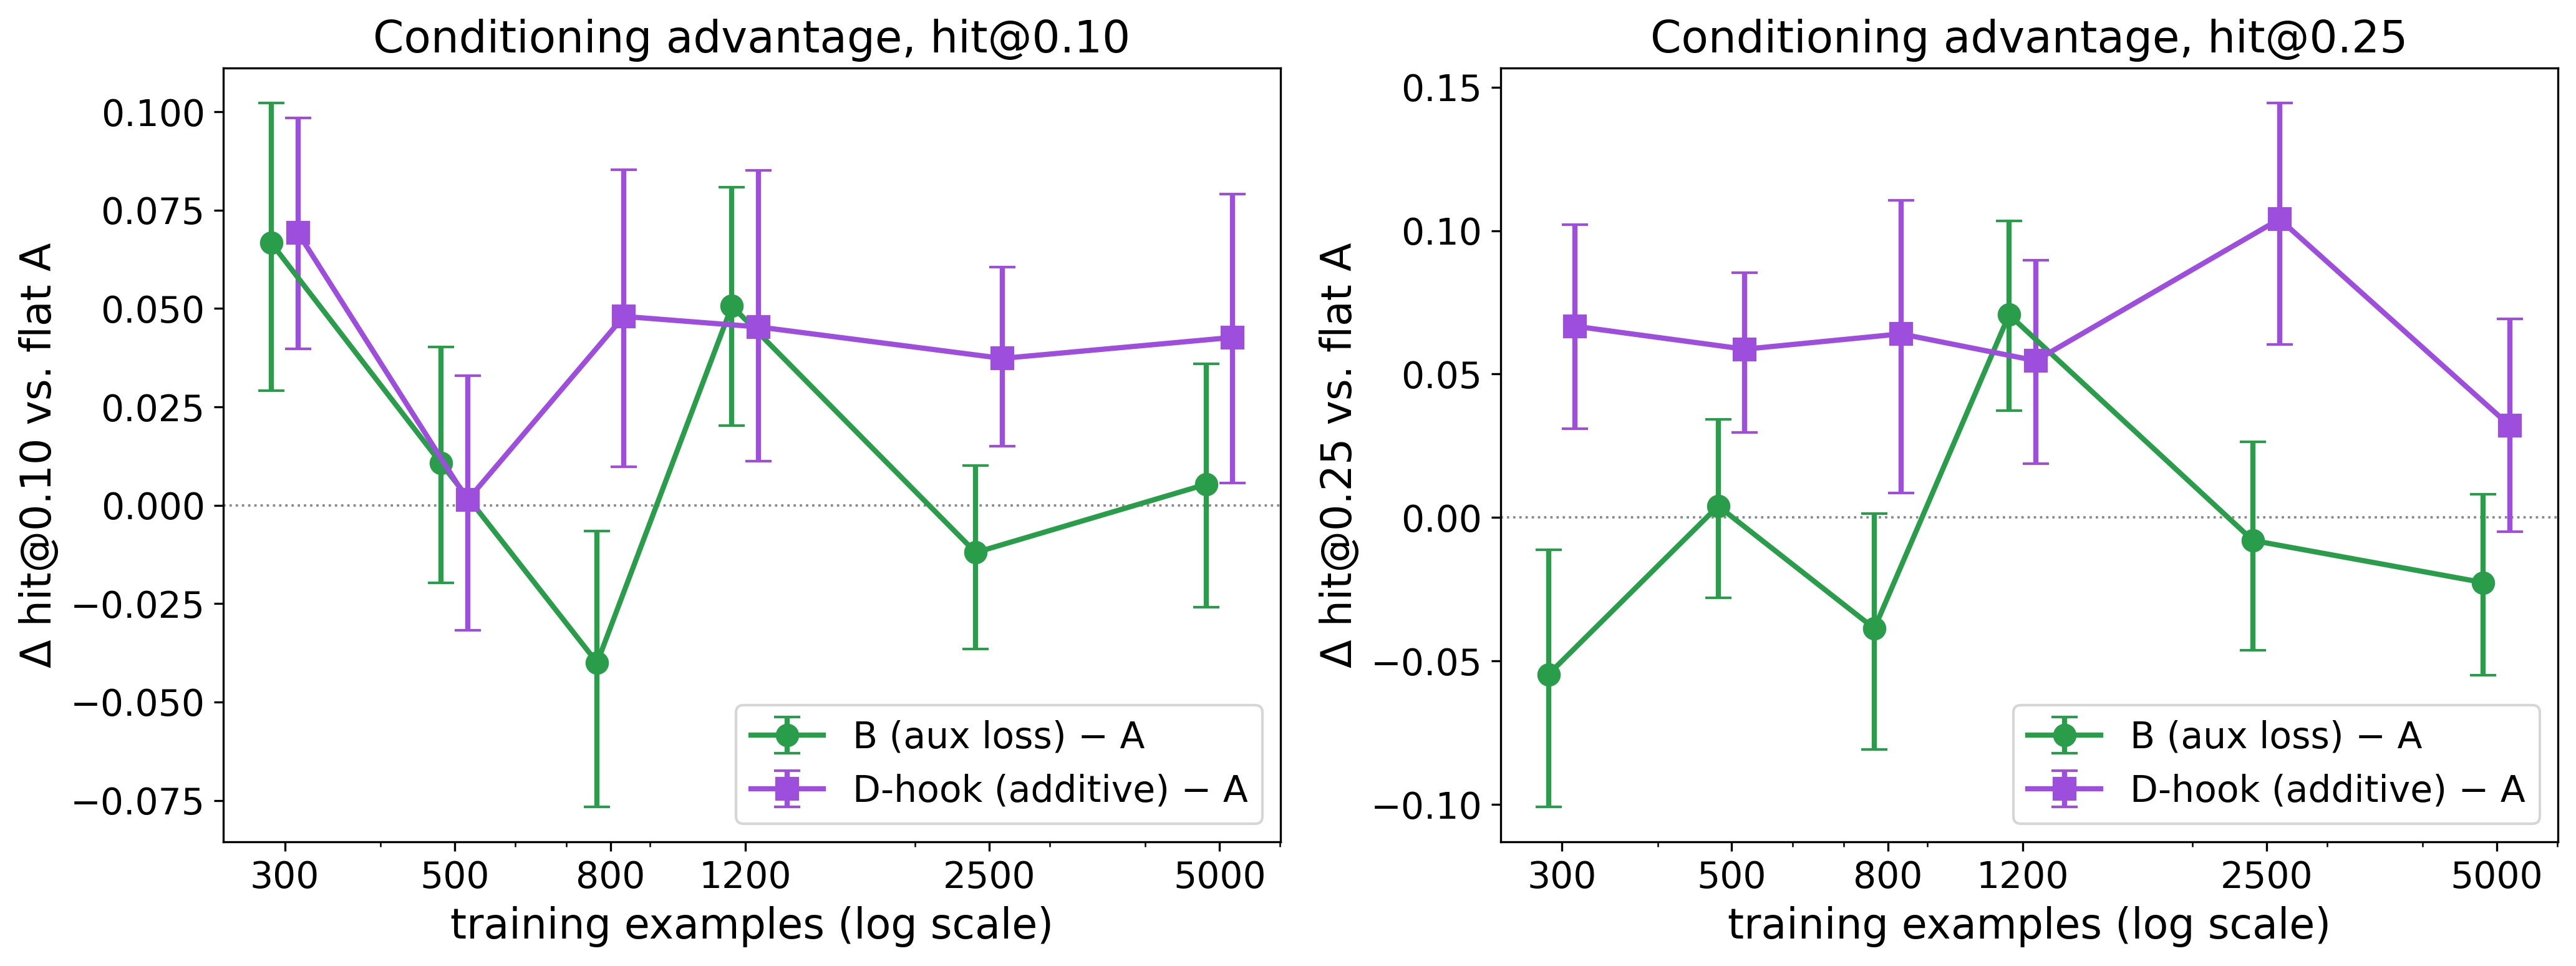
\includegraphics[width=0.96\linewidth]{scaling_curve_multiseed.png}
  \caption{Conditioning advantage over the flat baseline as a function of training-set size on \mix{all\_with\_coords}, three seeds per cell, 95\% paired-bootstrap intervals. Absolute accuracy (left) is not comparable across sizes because the validation slice moves with $n$; the within-size differences (center, right) are. D-hook is above zero at five of six sizes on \hitat{0.10} and at all six on \hitat{0.25}; B is above zero at two sizes and below at one. Full numbers in Table~\ref{tab:scaling}.}
  \label{fig:scaling}
\end{figure}

Figure~\ref{fig:scaling} extends the comparison to $n \in \{300, 500, 800, 1200, 2500, 5000\}$ with three seeds at every size. Two things change relative to the headline. First, the advantage of the auxiliary loss is not a general property: B beats A at 300 ($+0.067$) and 1,200 ($+0.051$), is indistinguishable from A at 500, 2,500, and 5,000, and is worse at 800 ($-0.040$, $p<0.01$). Second, D-hook's advantage persists: $+0.069$, $+0.001$, $+0.048$, $+0.045$, $+0.037$, and $+0.043$ \hitat{0.10} from smallest to largest, significant everywhere except at 500, and positive at every size on \hitat{0.25}. An earlier single-seed version of this curve suggested that the conditioning advantage shrinks with data; with three seeds, that is true of B and not of D-hook, whose gain at 5,000 examples ($+0.043$) is the same size as at 1,200. The two mechanisms tie at the headline size and differ everywhere else, and the difference favors the one that carries the action type into the forward pass.

Figure~\ref{fig:qualitative} in the appendix shows what the numbers look like on individual screens at the headline setting. Conditioning rescues some clicks that the baseline sends off-screen, and it also moves some correct clicks onto the wrong list item; on that seed the rescues outnumber the harms by 18 to 11 among 169 clicks, 45 clicks are correct under both models, and 90 are missed by both.

\section{Mechanism}
\label{sec:mechanism}

\subsection{A positional-encoding pitfall that produced a false negative}
\label{sec:mrope}
Our first implementation of the prepended token replaced the slot's embedding by constructing \texttt{inputs\_embeds} and passing that to the model instead of \texttt{input\_ids}. On \mix{taps\_and\_swipes} that variant scored $0.298 \pm 0.026$ \hitat{0.10} against $0.390 \pm 0.010$ for the flat baseline, a nine-point deficit with non-overlapping seeds, and we initially took it as evidence against conditioning. A diagnostic variant with the same slot but a frozen random embedding scored the same (0.290), which pointed at the injection path rather than the learned vector. Qwen2-VL computes its three-dimensional rotary positions from \texttt{input\_ids}, locating the image tokens in the id sequence to assign temporal, height, and width positions. Given \texttt{inputs\_embeds} instead, that computation does not see the same sequence, and the visual tokens are positioned as if the slot were not there, which corrupts the spatial layout the task depends on. D-hook and D-token keep \texttt{input\_ids} intact and modify embeddings through a forward hook; with that change the additive variant scored $0.392 \pm 0.043$ on the same control, a tie with the baseline, and the headline results followed. Any conditioning scheme that assembles \texttt{inputs\_embeds} for a model with multimodal positional encoding should verify that the position computation is unaffected, because the failure is silent and, in a two-billion-parameter model, large enough to invert a conclusion.

\subsection{Is the learned action embedding used at inference?}
\label{sec:causal}

\begin{table}[t]
\centering
\small
\caption{D-token causal-use test: the same trained model evaluated with the gold action embedding, a wrong (cyclically permuted) one, and a zeroed one (5 seeds, paired bootstrap over pooled examples).}
\label{tab:causal}
\resizebox{\linewidth}{!}{\begin{tabular}{lcccc}
\toprule
Conditioning & hit@0.05 & hit@0.10 & hit@0.25 & mean L2 $\downarrow$ \\
\midrule
gold & 0.140 $\pm$ 0.059 & 0.236 $\pm$ 0.058 & 0.502 $\pm$ 0.045 & 0.386 $\pm$ 0.020 \\
wrong & 0.014 $\pm$ 0.004 & 0.079 $\pm$ 0.013 & 0.200 $\pm$ 0.027 & 0.728 $\pm$ 0.081 \\
zero & 0.074 $\pm$ 0.055 & 0.167 $\pm$ 0.066 & 0.416 $\pm$ 0.103 & 0.489 $\pm$ 0.059 \\
\midrule
gold $-$ wrong & & +0.157 [+0.131, +0.182]$^{***}$ & +0.302 [+0.273, +0.331]$^{***}$ & -0.342 [-0.360, -0.324]$^{***}$ \\
gold $-$ zero & & +0.069 [+0.045, +0.092]$^{***}$ & +0.086 [+0.062, +0.109]$^{***}$ & -0.103 [-0.116, -0.090]$^{***}$ \\
\bottomrule
\end{tabular}}
\end{table}


D-token's failure to help could mean the model ignores the slot. Table~\ref{tab:causal} rules that out. We evaluate each trained D-token model (five seeds, 1,250 pooled examples) three times on the same validation set: with the gold action embedding, with a wrong one obtained by cyclically permuting the classes present (click to type, type to scroll, scroll to click), and with the embedding table zeroed. The wrong embedding drops \hitat{0.10} from 0.236 to 0.079 and the zeroed one to 0.167; both differences exclude zero at $p<0.001$. The learned vector has norm 2.2 and the model obeys it. The cyclic permutation sends most examples (clicks) to \emph{type}, whose training targets are the degenerate coordinate, so part of the wrong-embedding drop is the model dutifully emitting that coordinate; the zeroed condition has no such confound and still costs seven points. Section~\ref{sec:attention} adds a wrong map that swaps only clicks and scrolls and finds a similar collapse. D-token is therefore used and not enough: the refutation is of the mechanism's usefulness, not of its activity.

\subsection{Where the model looks, and whether the signal is needed at inference}
\label{sec:attention}

\begin{figure}[t]
  \centering
  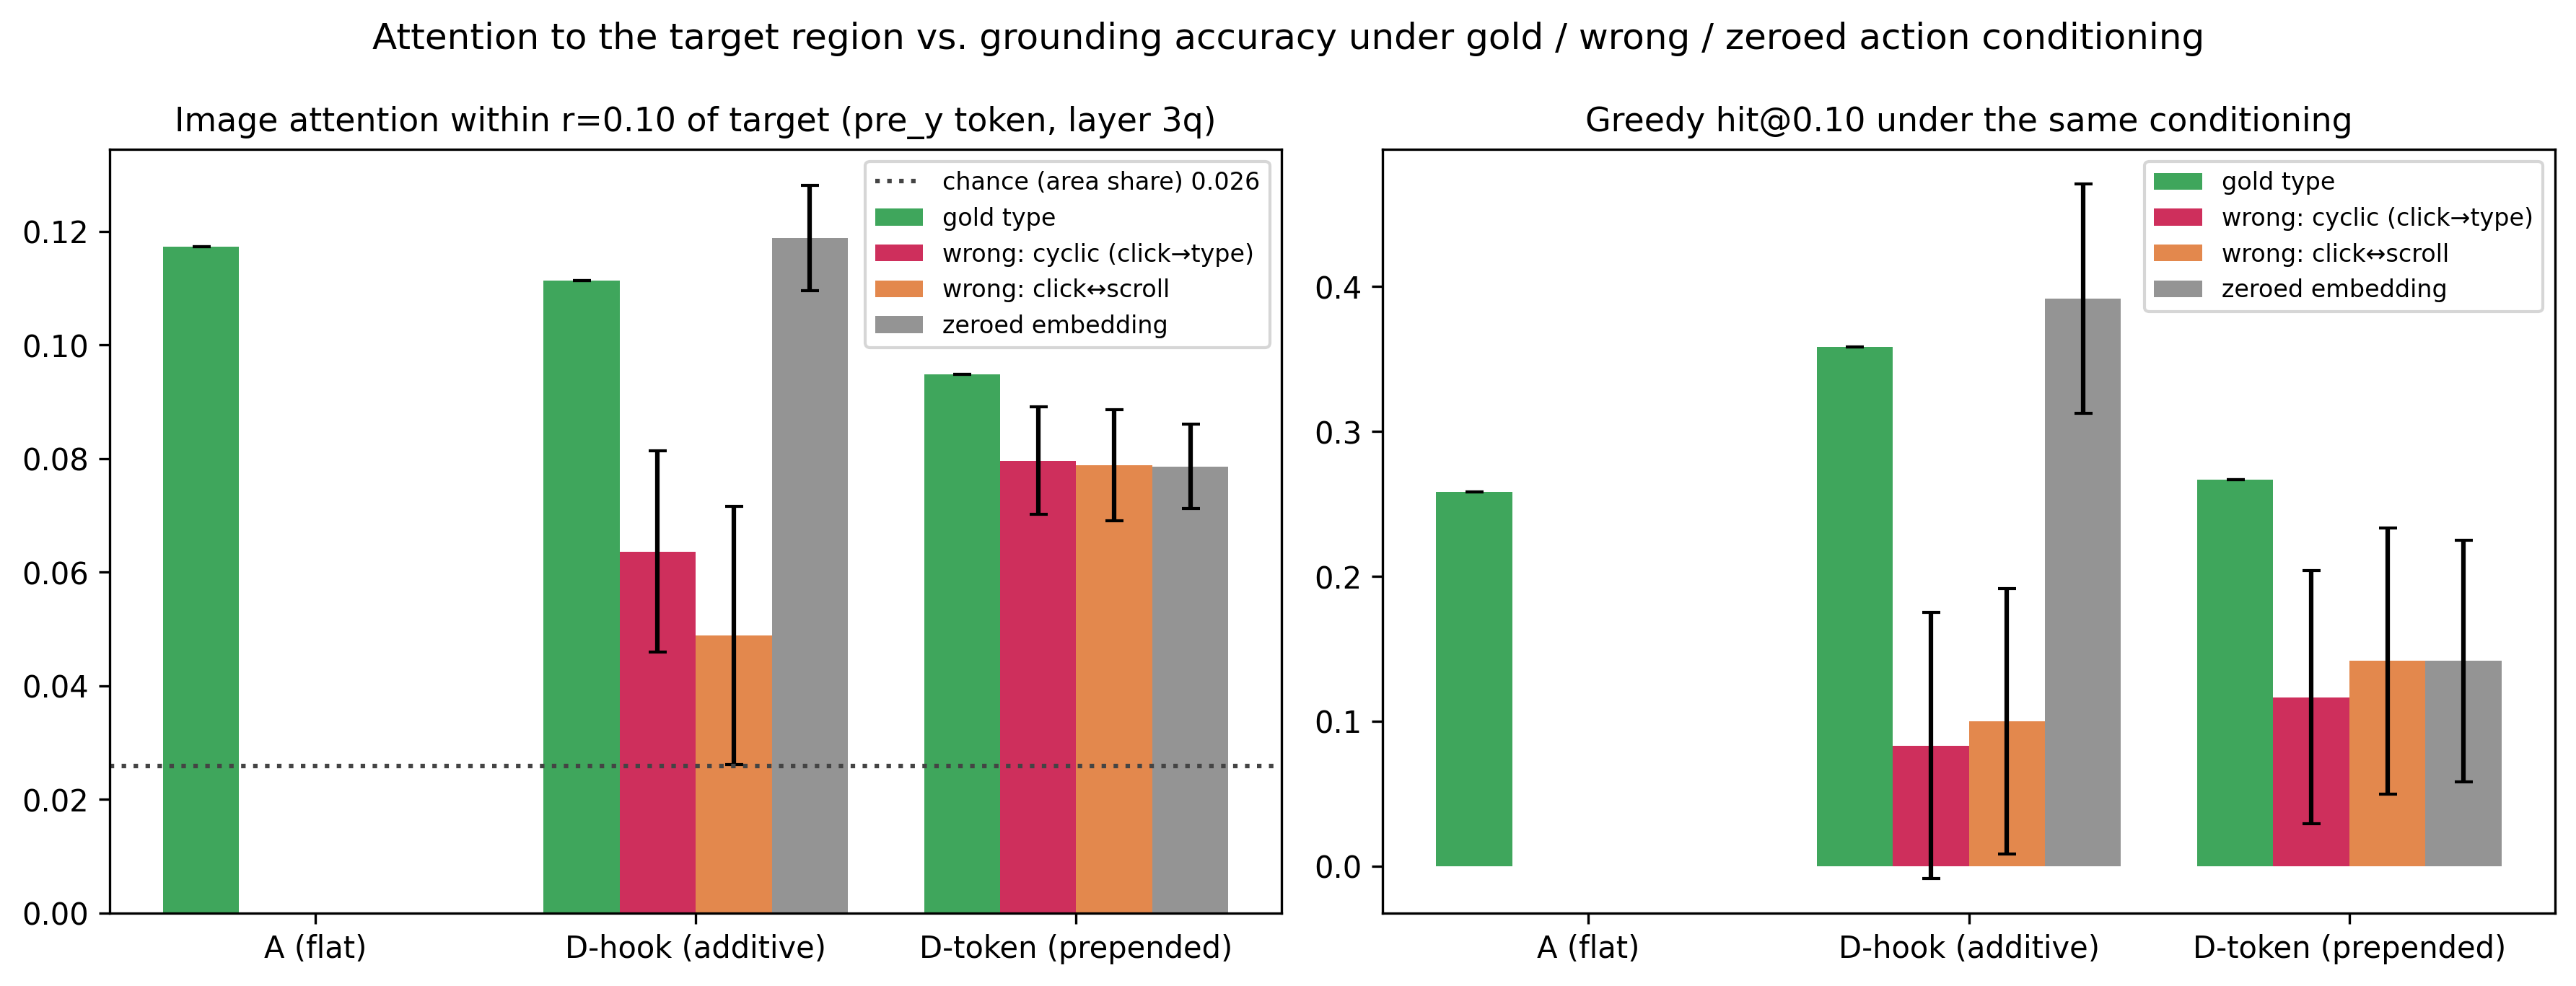
\includegraphics[width=0.92\linewidth]{attn_aggregate.png}
  \caption{Same trained model, four conditionings, 120 validation screens, one seed per variant. Left: share of image attention within $0.10$ of the target from the token that predicts the y coordinate (3/4-depth layer, head-averaged); the dotted line is the share of image tokens within that radius. Right: greedy \hitat{0.10} under the same conditioning. Error bars are 95\% paired-bootstrap intervals of the difference from gold. Zeroing the additive embedding changes nothing; zeroing the prepended token costs accuracy and attention.}
  \label{fig:attn}
\end{figure}

\begin{table}[t]
\centering
\footnotesize
\caption{Where the model looks, and whether it matters. Share of the y-predicting token's image attention within 0.10 of the gold target (3/4-depth layer; chance is 0.026) and greedy hit@0.10 under gold, wrong and zeroed action conditioning on the first 120 validation examples, one seed per model. $\Delta$ = gold $-$ condition with 95\% paired-bootstrap CI.}
\label{tab:attn}
\resizebox{\linewidth}{!}{\begin{tabular}{llcccc}
\toprule
Model & Conditioning & target attn.\ & $\Delta$ vs.\ gold & hit@0.10 & $\Delta$ vs.\ gold \\
\midrule
A (flat) & gold type & 0.117 &  & 0.258 &  \\
\midrule
D-hook (additive) & gold type & 0.111 &  & 0.358 &  \\
 & wrong (cyclic) & 0.064 & +0.048 [+0.030, +0.065]$^{***}$ & 0.083 & +0.275 [+0.183, +0.367]$^{***}$ \\
 & wrong (click$\leftrightarrow$scroll) & 0.049 & +0.062 [+0.040, +0.086]$^{***}$ & 0.100 & +0.258 [+0.167, +0.350]$^{***}$ \\
 & zeroed & 0.119 & -0.008 [-0.017, +0.001] & 0.392 & -0.033 [-0.117, +0.042] \\
\midrule
D-token (prepended) & gold type & 0.095 &  & 0.267 &  \\
 & wrong (cyclic) & 0.080 & +0.015 [+0.006, +0.025]$^{**}$ & 0.117 & +0.150 [+0.058, +0.233]$^{**}$ \\
 & wrong (click$\leftrightarrow$scroll) & 0.079 & +0.016 [+0.006, +0.026]$^{**}$ & 0.142 & +0.125 [+0.033, +0.217]$^{**}$ \\
 & zeroed & 0.079 & +0.016 [+0.009, +0.024]$^{***}$ & 0.142 & +0.125 [+0.042, +0.208]$^{**}$ \\
\bottomrule
\end{tabular}}
\end{table}


To separate training-time from inference-time effects we repeat the intervention for D-hook, add a second wrong map that swaps clicks and scrolls (and sends the ungroundable type class to click), and measure attention at the same time (Figure~\ref{fig:attn}, Table~\ref{tab:attn}). For attention we teacher-force the gold answer and read the head-averaged attention row of the token whose next prediction is the first digit of the y coordinate, at the layer three quarters of the way through the network; the share of that row's image mass falling within $0.10$ of the target is our localization measure, and the share of image tokens within that radius (0.026) is chance. Under gold conditioning, both models put 10 to 11\% of that token's image attention on the target region, four times chance, so the coordinate is grounded in the right part of the screen when it is right. The last prompt token, which earlier visualizations used, localizes far less (about 4\%) under every conditioning; localization happens once the x coordinate has been emitted.

The two mechanisms diverge on the interventions. For D-hook, zeroing the embedding leaves attention (0.119 vs.\ 0.111) and accuracy (0.392 vs.\ 0.358) unchanged or slightly higher, while either wrong map roughly halves the target attention and drops \hitat{0.10} to 0.08 to 0.10. The model reads the additive signal, and it has also learned, through the LoRA weights, to do without it; the benefit is a training effect and the signal is redundant at test time unless it lies. For D-token, zeroing costs both attention ($0.095 \to 0.079$, $p<0.001$) and accuracy ($0.267 \to 0.142$, $p<0.01$), as much as a wrong type does. The prepended token is consulted at inference, and consulting it does not make the model better than a baseline that never saw an action type. Together with Section~\ref{sec:scaling}, this explains the ranking: the value of action-type supervision here is what it teaches the adapter weights, and mechanisms that deliver it as a training signal (B) or as a redundant additive one (D-hook) capture it, while a mechanism that makes the model depend on the signal at inference (D-token) does not.

\section{Limitations}
\label{sec:limitations}
The study is deliberately small. One backbone at 2B parameters, LoRA adapters only, validation slices of 200 to 250 steps, and one L4 per run mean that the absolute grounding numbers are far below the field's leaderboards and that per-seed variance is large; the conclusions rest on paired statistics over pooled examples rather than on any single run. AITW's type events are ungroundable, so the ``spatially informative'' mix is in effect a click-versus-scroll-versus-type discrimination. The attention analysis in Section~\ref{sec:attention} uses one seed per variant and one layer; the y-predicting token was chosen after observing that the last prompt token does not localize, and all positions are reported in the appendix. Mind2Web is a control rather than a target, and we do not evaluate on ScreenSpot or on long-horizon task success, where the compounding-error argument of the introduction would have to be tested directly. The mechanisms are compared at one learning rate and one adapter configuration; a stronger D-token could exist under a different schedule for the embedding table.

\section{Conclusion}
\label{sec:conclusion}
Telling a small grounding model which action it is grounding helps when the action type says something about where the target is, and does nothing when it does not. The help comes from training, not from the signal at inference: an auxiliary loss captures it at the headline size, an additive embedding that the model can ignore at test time captures it at every size we tried, and the prepended token we set out to validate is used by the model and improves nothing. For practitioners adapting small VLMs as GUI agents, the lessons are to supervise the action type during adaptation, to prefer conditioning the model does not depend on at inference, and to check position ids whenever \texttt{inputs\_embeds} is on the path.

\begin{ack}
Acknowledgments are omitted for review.
\end{ack}

\bibliographystyle{plainnat}
\bibliography{references}

\clearpage
\appendix

\section{Training and evaluation details}
\label{app:details}
\paragraph{Data.} AITW screenshots in the mirror we use are stored as raw RGB byte buffers without an image header; we decode them by matching the buffer length against seven observed resolutions (for example $540\times1140$ and $412\times732$) with a portrait-aspect fallback. Mind2Web screenshots are downscaled so that no image exceeds one megapixel. Examples are drawn from the AITW training stream in order, filtered to the mix's action labels; the first $n$ eligible steps form the training slice and the next 250 (200 for the control mix) form validation.

\paragraph{Prompts.} Stage~2 prompts contain the screenshot, the line \texttt{Goal: \{goal\}}, and the instruction \texttt{Predict the action coordinate.} (C uses \texttt{Predict the action type and coordinate.} and is trained to answer with the action word before the coordinate). D-token places \texttt{<|action\_slot|>} at the start of the text; exactly one slot per sequence is asserted at every step.

\paragraph{Compute.} Everything runs on single NVIDIA L4 GPUs. A Stage-2 run at 1,200 training examples takes about 35 minutes; the full study, including the runs that were later retracted, cost under 100 GPU-hours.

\paragraph{Optimization.} AdamW with learning rate $2\times10^{-5}$ and weight decay 0.01, batch size 1, gradient clipping at 1.0, two epochs, a fixed per-epoch shuffle seeded by the run seed. The action-embedding table (D-hook, D-token) and the auxiliary head (B) share the base learning rate. D-hook's table is zero-initialized; D-token's uses $\mathcal{N}(0, 0.02^2)$. Evaluation is greedy with at most 16 new tokens; the coordinate is parsed with a regular expression and an unparseable output counts as a miss at distance $\sqrt{2}$.

\paragraph{Statistics.} For each comparison we pool per-example distances over the seeds that both variants share, resample the pooled units with replacement 10,000 times, and report the percentile interval and the two-sided bootstrap $p$-value of the mean difference; a paired sign-permutation test with 10,000 permutations is run alongside and agrees with the bootstrap in every case in the paper. Pooled units from the same example under different seeds are correlated, which makes the intervals somewhat optimistic; the permutation test is affected in the same way.

\section{Stage 1 and per-class tables}
\label{app:tables}

\begin{table}[h]
\centering
\small
\caption{Stage~1 action-type macro-F1 (three seeds). On Mind2Web the instruction names the action, so the screenshot adds little; on AITW the instruction describes a goal and the screenshot is what separates the classes.}
\label{tab:stage1}
\begin{tabular}{lcc}
\toprule
Features & Mind2Web (2 classes) & AITW (5 classes) \\
\midrule
text only & $0.597 \pm 0.011$ & $0.141 \pm 0.032$ \\
text + screenshot & $0.605 \pm 0.016$ & $0.555 \pm 0.036$ \\
zeroed (sanity) & $0.469 \pm 0.000$ & $0.110 \pm 0.051$ \\
\midrule
TF-IDF + logistic regression & $0.622$ & $0.168$ \\
majority class & $0.472$ & $0.140$ \\
\bottomrule
\end{tabular}
\end{table}

\begin{table}[h]
\centering
\small
\caption{Per-class \hitat{0.10} on the headline mix (five seeds). AITW \emph{type} events carry a degenerate touch coordinate (mean distance $\sqrt{2}$ for every model), so the class is ungroundable and contributes a constant. The conditioning gain is a \emph{click} gain; only D-hook also improves \emph{scroll}.}
\label{tab:perclass}
\begin{tabular}{lccc}
\toprule
Variant & click ($n{=}169$) & scroll ($n{=}46$) & type ($n{=}35$) \\
\midrule
A: flat & $0.256 \pm 0.062$ & $0.304 \pm 0.034$ & $0.000$ \\
B: aux.\ loss & $0.357 \pm 0.026$ & $0.278 \pm 0.018$ & $0.000$ \\
C: hard routing & $0.356 \pm 0.065$ & $0.172 \pm 0.076$ & $0.000$ \\
D-hook: additive & $0.321 \pm 0.064$ & $0.357 \pm 0.039$ & $0.000$ \\
D-token: prepended & $0.269 \pm 0.069$ & $0.304 \pm 0.090$ & $0.000$ \\
\bottomrule
\end{tabular}
\end{table}

\section{Full scaling table}
\label{app:scaling}
\begin{table}[t]
\centering
\small
\caption{Conditioning advantage vs.\ training-set size (AITW \texttt{all\_with\_coords}, 3 seeds per cell, paired bootstrap over pooled (seed, example) units). Absolute values are not comparable across rows because the validation slice moves with $n$.}
\label{tab:scaling}
\resizebox{\linewidth}{!}{\begin{tabular}{rccccc}
\toprule
$n_{\text{train}}$ & A hit@0.10 & B $-$ A & D-hook $-$ A & B $-$ A (hit@0.25) & D-hook $-$ A (hit@0.25) \\
\midrule
300 & 0.139 $\pm$ 0.032 & +0.067 [+0.037, +0.096]$^{***}$ & +0.069 [+0.044, +0.095]$^{***}$ & -0.055 [-0.080, -0.031]$^{***}$ & +0.067 [+0.044, +0.091]$^{***}$ \\
500 & 0.315 $\pm$ 0.059 & +0.011 [-0.015, +0.036] & +0.001 [-0.027, +0.029] & +0.004 [-0.020, +0.029] & +0.059 [+0.031, +0.087]$^{***}$ \\
800 & 0.261 $\pm$ 0.020 & -0.040 [-0.069, -0.011]$^{**}$ & +0.048 [+0.017, +0.080]$^{**}$ & -0.039 [-0.065, -0.012]$^{**}$ & +0.064 [+0.036, +0.092]$^{***}$ \\
1200 & 0.255 $\pm$ 0.026 & +0.051 [+0.024, +0.079]$^{***}$ & +0.045 [+0.017, +0.073]$^{**}$ & +0.071 [+0.041, +0.100]$^{***}$ & +0.055 [+0.025, +0.084]$^{***}$ \\
2500 & 0.244 $\pm$ 0.037 & -0.012 [-0.035, +0.011] & +0.037 [+0.013, +0.063]$^{**}$ & -0.008 [-0.037, +0.020] & +0.104 [+0.075, +0.133]$^{***}$ \\
5000 & 0.363 $\pm$ 0.009 & +0.005 [-0.021, +0.032] & +0.043 [+0.016, +0.069]$^{**}$ & -0.023 [-0.044, +0.000] & +0.032 [+0.008, +0.056]$^{*}$ \\
\bottomrule
\end{tabular}}
\end{table}


\section{Attention at every probe position}
\label{app:attention}
Table~\ref{tab:attn} reports the token that predicts the y coordinate. Table~\ref{tab:attn_positions} gives the same measure for the last prompt token (the one that predicts the opening parenthesis) and for the token that predicts the first x digit, at the 3/4-depth layer. The last prompt token barely localizes under any conditioning, the x-predicting token localizes weakly, and the y-predicting token is where the target region receives attention.

\begin{table}[h]
\centering
\small
\caption{Share of image attention within $0.10$ of the target (chance $0.026$) at three probe positions, seed 42, 120 screens, 3/4-depth layer. Contrasts are gold minus condition with 95\% paired-bootstrap intervals.}
\label{tab:attn_positions}
\begin{tabular}{llcccc}
\toprule
Model & Position & gold & wrong (cyclic) & wrong (click$\leftrightarrow$scroll) & zero \\
\midrule
D-hook & last prompt token & 0.040 & 0.036 & 0.035 & 0.036 \\
D-hook & pre-x token & 0.039 & 0.036 & 0.037 & 0.039 \\
D-hook & pre-y token & 0.111 & 0.064 & 0.049 & 0.119 \\
D-token & last prompt token & 0.038 & 0.034 & 0.034 & 0.035 \\
D-token & pre-x token & 0.038 & 0.034 & 0.033 & 0.035 \\
D-token & pre-y token & 0.095 & 0.080 & 0.079 & 0.079 \\
\bottomrule
\end{tabular}
\end{table}

\section{Qualitative examples}
\label{app:qual}
\begin{figure}[h]
  \centering
  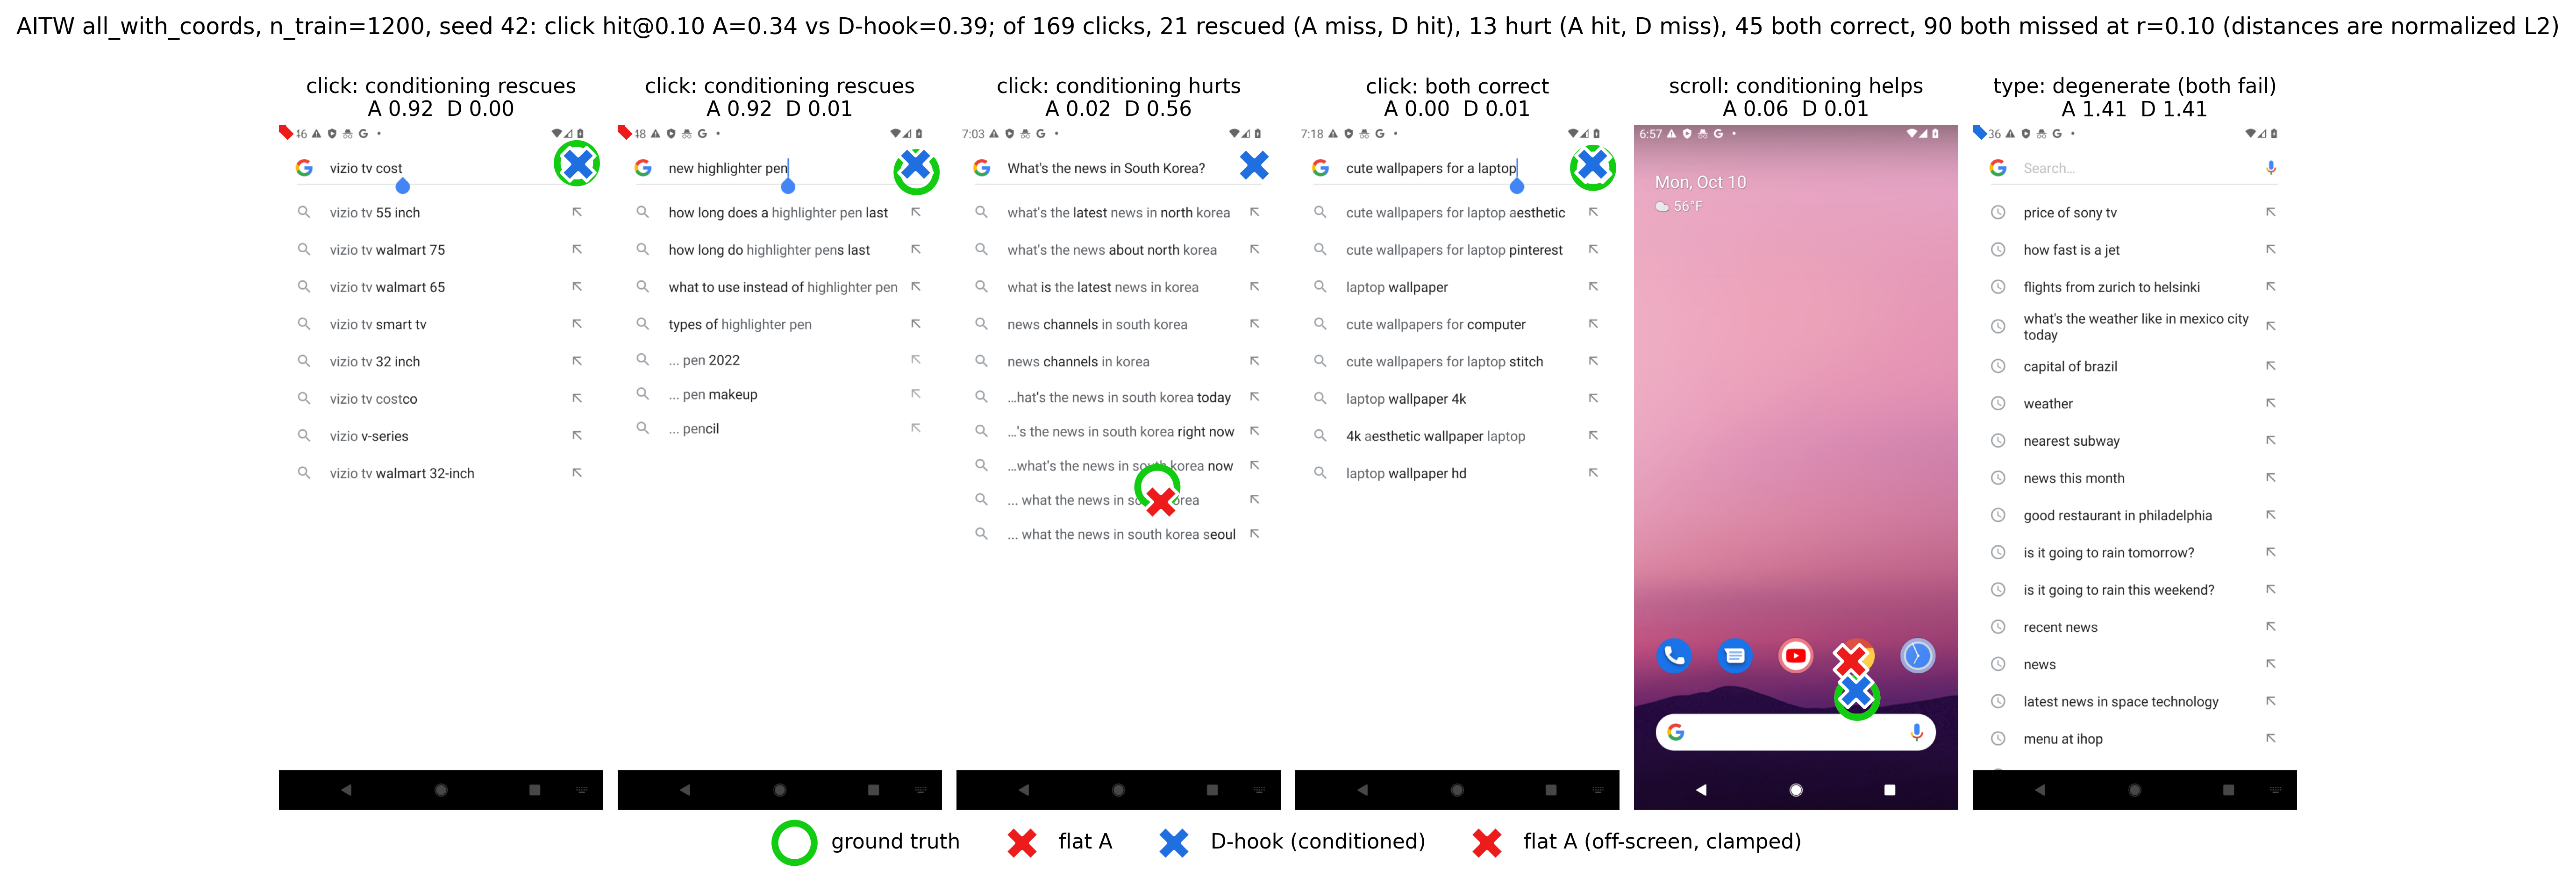
\includegraphics[width=\linewidth]{qualitative_v2_1x6.png}
  \caption{Predictions of the flat baseline (red) and D-hook (blue) against the target (green) on held-out AITW screens at the headline setting, one seed. The panels are a fixed spread of outcomes rather than a selection of wins: two rescues, a case where conditioning hurts, a case where both are right, a scroll, and a degenerate \emph{type} example on which both models miss at distance $\sqrt{2}$. The title reports the base rates on this seed. In the rescue panels the baseline's prediction is off-screen and drawn clamped at the corner.}
  \label{fig:qualitative}
\end{figure}

\begin{figure}[h]
  \centering
  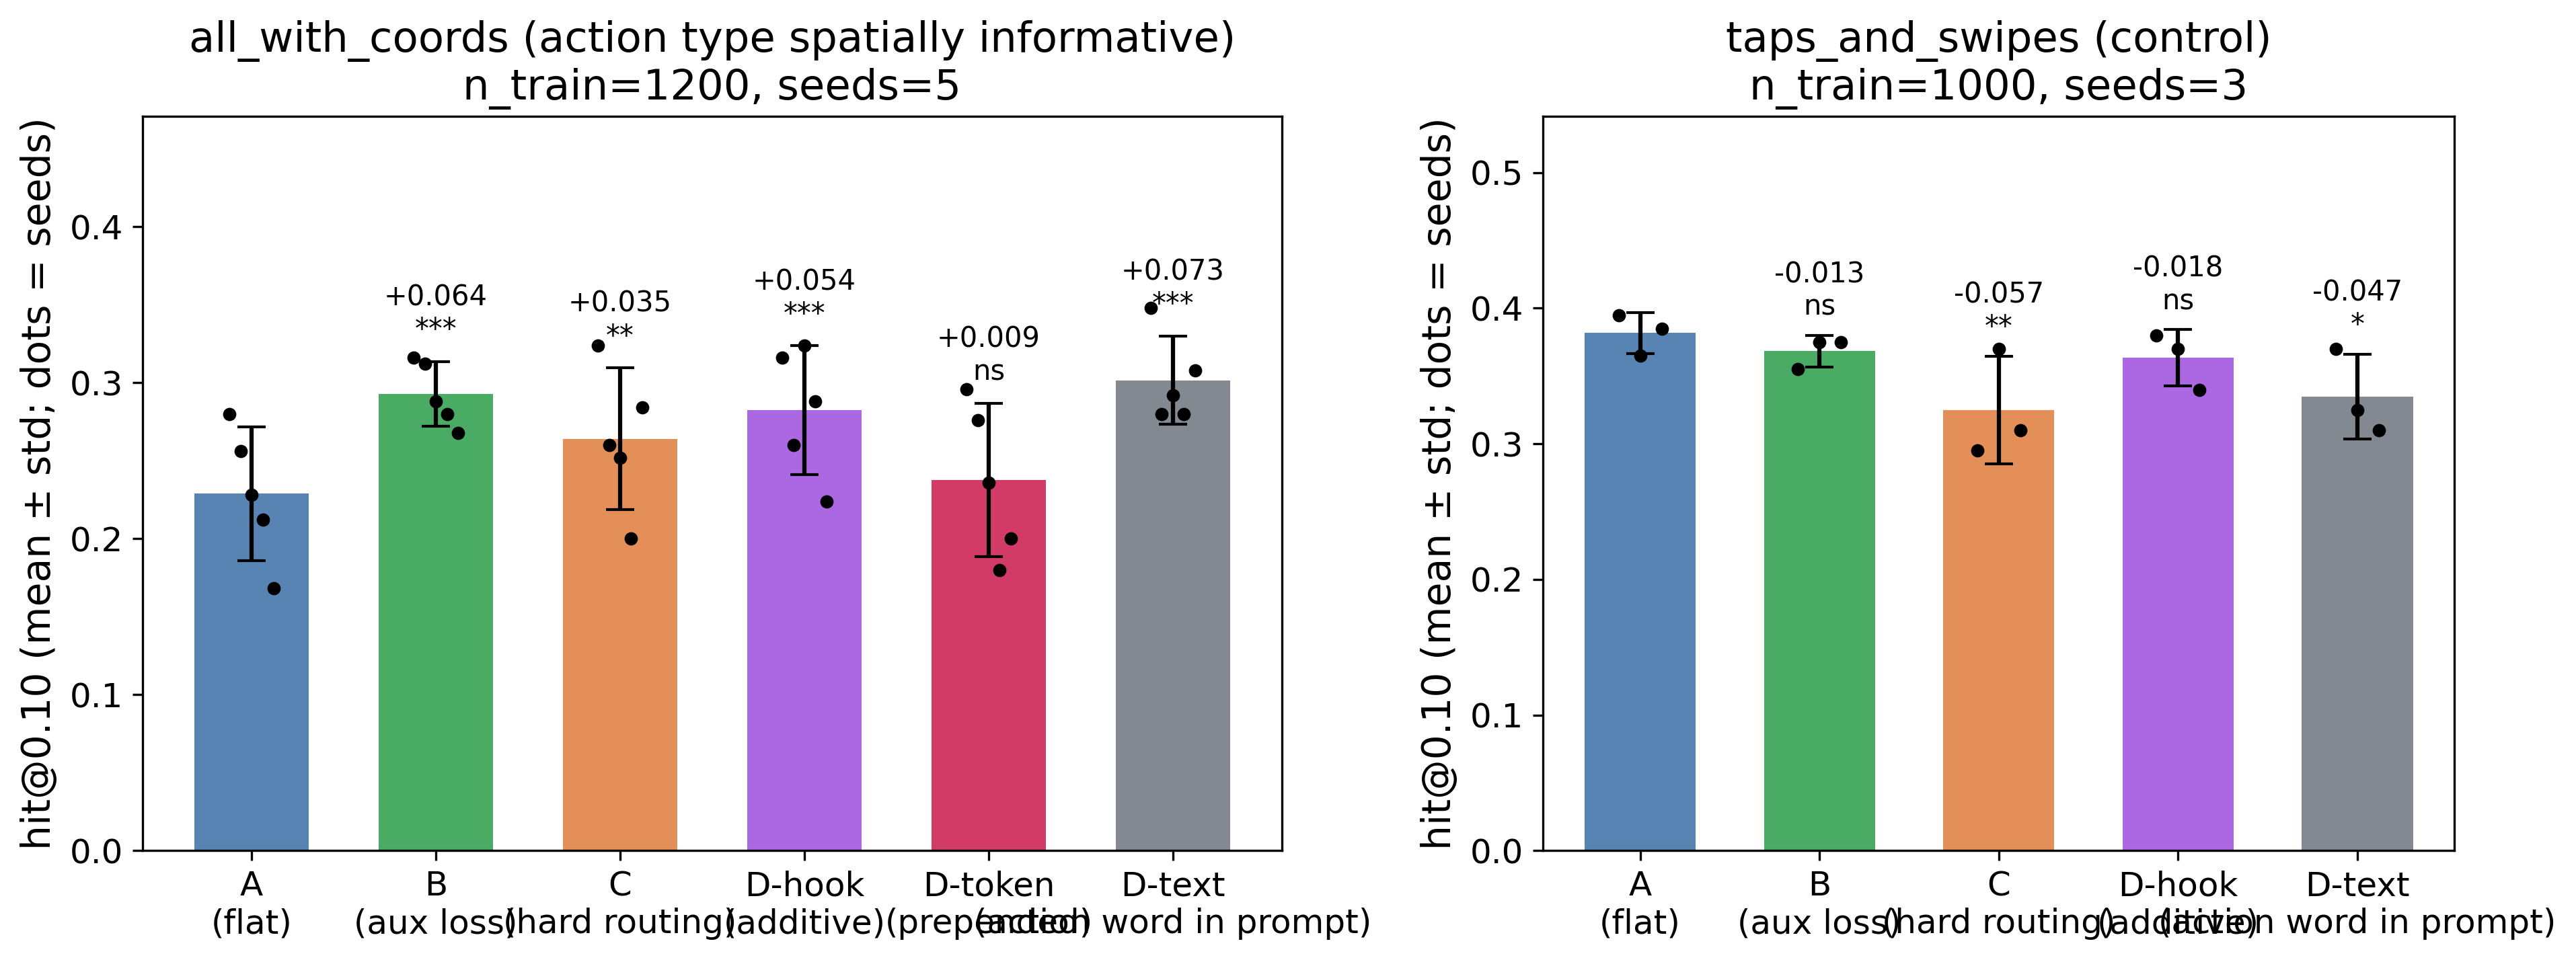
\includegraphics[width=\linewidth]{ablation_headline_vs_control.png}
  \caption{\hitat{0.10} per variant on the headline mix (left, five seeds) and the control mix (right, three seeds), with individual seeds as dots and the paired-bootstrap difference from the flat baseline above each bar.}
  \label{fig:bars}
\end{figure}

\end{document}
